\section{Elektronen im Festkörper} \label{kap:5}

Erinnerung adiabatische Näherung (Born-Oppenheimer-Näherung):\\
Elektronenbeugung und Gitterdynamik werden getrennt behandelt.
\begin{itemize}
    \item Bewegung der Valenzelektronen im \textbf{statischen} Potential des Gitters. (positiv geladene Ionenrümpfe)
    \item Bei Transportprozessen von Elektronen:
    Elektronen-Gitter-WW als Strömung betrachtet.
\end{itemize}

Weitere Vereinfachungen:
\begin{itemize}
    \item \textbf{Ein-Elektron-Näherung:} Betrachte einzelnes Elektron im statischen Potential gegeben durch Ionenrümpfe und alle anderen Elektronen.
    \begin{itemize}
        \item[$\rightarrow$] Vernachlässigung $e^-$-$e^-$-WW, die über statisches Potiential hinausgeht. Beispiel für $e^-$-$e^-$-WW: Magnetismus, Supraleitung.
    \end{itemize}
    \item Beachtung des Pauliprinzips: Zustände werden sukzessive aufgefüllt
    \begin{itemize}
        \item[$\rightarrow$] unabhängige Elektronen  
    \end{itemize}    
\end{itemize}

\subsection{Das freie Elektronengas} \label{kap:5_1}
Zunächst zusätzliche Vernachlässigung der Gitterperiodizität
\begin{itemize}
    \item[$\rightarrow$] einzelnes Elektron im konstanten Potentialtopf (Sommerfeld-Modell)
    \begin{figure}[H]
        \centering
        \input{figures/5_1Grapht.tex}
        \label{5_1Graph}
    \end{figure}
    \item Beschreibung der Elektronen im Festkörper als \textbf{freies Elektronengas}
    \item Potentialtopf begrenzt durch Festkörper. Oberer Rand entspricht Vakuumzustand (im Folgenden als $\infty$ angenommen)
    \item Gute Näherung für \glqq einfache Metalle\grqq (Alkalimetalle, Münzmetalle)
    \item Keine gute Näherung für die Übergangsmetalle
\end{itemize}

\begin{itemize}
    \item [(a)] \textbf{Schrödinger-Gleichung in 3D} \\
        \begin{align}
            \frac{-\hbar^2}{2m} \Delta \Psi(\textbf{r}) + V(\textbf{r}) \Psi(\textbf{r}) = E \Psi(\textbf{r})
        \end{align}
        mit Potential
        \begin{align*}
            V(\textbf{r}) = \begin{cases}
                0 & \text{für } 0 \le x,y,z \le L\\
                \infty & sonst
            \end{cases}
        \end{align*}
        Ansatz: Ebene Wellen $ \Psi(\textbf{r}) = \frac{1}{\sqrt{V}} e^{i\textbf{kr}}$  \\
        Energieeigenwert des Grundzustandes:
        \begin{align}
            E = \frac{\hbar^2k^2}{2m} = \frac{\hbar^2}{2m}(k_x^2 + k_y^2 + k_z^2)
        \end{align}
        Periodische Randbedingungen:\\ $\Psi(x,y,z) = \Psi(x+L,y,z) = \Psi(x,y+L,z) = \Psi(x,y,z+L)$ \\
        $\rightarrow$ $k_i = \frac{2\pi}{L} \cdot m_i $ mit $m_i$ für $i =x,y,z$ ganzzahlig. \\
        diskret aber \glqq liegen dicht \grqq d.h. quasikontinuierlich für große L. \\
        Für niedrigdimensionale Festkörper wird Schrödingergleichung mit Ansatz ebener Wellen für \glqq vorhandene Dimension\grqq  und als stehene Welle für \glqq nicht vorhandene Dimension \grqq  mit Wellenlänge $ \lambda_i = \frac{2d}{i} $. ($d$ : Abmessung in nicht vorhandener Dimension) \\
        
    \textbf{2D Zweidimensionales Elektronengas:} \\
        Z.B. dünne Metallfaden, 2DEG im Halbleiter-Heterostrah (Si-integrierte Schaltung) mit Dicke $d$
    \begin{align*}
        \lambda_i = \frac{2d}{i} \text{ oder } k_{i,z} = \frac{2\pi}{\lambda_i} = \frac{\pi}{d}i
    \end{align*}
    Schrödingergleichung mit
    \begin{align*}
        V(\textbf{r}) = \begin{cases}
                0 &\text{für } 0 \leq x,y \leq L\\
                \infty & \text{sonst}
            \end{cases}
    \end{align*}
    Ansatz 
    \begin{align*}
        \Phi(x,y,z) = \frac{1}{\sqrt{V}}\sin(k_z,it)\cdot e^{i k_x x}
    \end{align*}
    Eigenwerte
    \begin{align*}
        E = \frac{\hbar^2 k_{\Phi}^2}{2m} + \hbar^2 \frac{k_y^2}{2m} + \frac{i^2\hbar^2}{8md^2} \text{ mit } E_i = 8md^2
    \end{align*}
    Für $d\leq 5$mm werden tranversale Energien $E_i$ nicht vernachlässigt $\rightarrow$ 2D Subbänder: Parabeln in $k_x$- und $k_y$-Richtung.
    
    \textbf{2D Zweidimensionales Elektronengas:} \\
    1D Nanodraht mit quadratischen Querschnitt $\rightarrow$ Übungsauffgabe zu Lösen
    \begin{figure}[]
        \centering
        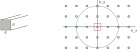
\includegraphics[]{figures/5_1Balken_Gitter.pdf}
        \caption{Die Dichte der erlaubten Wellenvektoren im k-Raum}
        \label{}
    \end{figure}
    \begin{itemize}
        \item 3D: $\delta^{3D}(k) = \frac{1}{\left(\frac{2\pi}{2}\right)} = \frac{V}{(2\pi)^3}$
        \item 2D: $\delta^{2D}(k) = \frac{A}{(2\pi)^2}$
        \item 1D: $\delta^{1D}(k) = \frac{L}{(2\pi)^1}$
    \end{itemize}
    \item[(b)] \textbf{Zustandsdichte} \\
        Zustandsdichte im Impulsraum: \\
        Die Dichte der erlaubten Wellenvektoren im k-Raum:
        \begin{align}
            3D \text{ : } \rho(k) &= \frac{1}{\left(\frac{2\pi}{L}\right)^3} &&= \frac{V}{(2\pi)^3} \\
            2D \text{ : } \rho(k) &= \dots &&= \frac{A}{(2\pi)^2} \\
            1D \text{ : } \rho(k) &= \dots &&= \frac{L}{(2\pi)^1}
        \end{align}
        Pauliprinzip: jeder k-Zustand kann doppelt besetzt werden wegen Spin: \\
        $\rightarrow$ $ 3D : D(k) = \frac{V}{(2\pi)^3} $ , $ 2D : \dots $  \\
        Zustandsdichte im Energieraum (analog zu Kap.4) in 3D:
        \begin{align}
            D(E)\mathrm{d} \approx \int_E^{E+\mathrm{d}E} D(E)\mathrm{d}E &= \int_{k(E)}^{k(E+\mathrm{d}E)} D(k)\mathrm{d}^3k = \frac{2V}{(2\pi)^3} \int_{k(E)}^{k(E+\mathrm{d}E)} \mathrm{d}^3k \\
            &= \frac{2V}{(2\pi)^3} \cdot 4 \pi k^2 \mathrm{dk}
        \end{align}
        wobei im letzten Schritt ausgenutzt wurde, dass $E = const$ auf Kugelfläche. \\
        Ausdrücken durch Energie: $ E = \frac{\hbar^2k^2}{2m} \rightarrow k = \sqrt{\frac{2mE}{\hbar^2}}$ und damit $ \frac{\mathrm{d}E}{\mathrm{d}k} = \frac{\hbar^2k}{m}$ \\
        $\rightarrow D(E) = \frac{V}{2\pi^2}\left(\frac{2m}{\hbar^2}\right)^{3/2}\sqrt{E} \propto \sqrt{E}$. \\
        \textbf{2D:} $D_i(E) = \frac{A}{2\pi}\frac{2m}{\hbar^2} = const $ ab $E \ge E_i$ \\
        $D^{2D}(E) = \sum_i D_i(E)$ \\
        \textbf{1D:} $D_{ij}(E) = \frac{L}{\pi}\left(\frac{2m}{\hbar^2}\right)^{1/2}\frac{1}{\sqrt{E}} \propto \frac{1}{\sqrt{E}} $ für $ E > E_{ij}$ \\
        $D^{1D}(E) = \sum_{i,j} D_{ij}(E)$
        \begin{figure}[H]
            \centering
            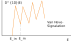
\includegraphics[]{figures/5_1zigzack.pdf}
            \caption{}
            \label{}
        \end{figure}
        
        Zustandsdichte und Dispersion des Fermigases
        % \begin{figure}[H]
        %     \centering
        %     \includegraphics[width=0.8\textwidth]{figures/5_zdfermi}
        %     \caption{}
        %     \label{fig:5_zdfermi}
        % \end{figure}

    \item[(c)] \textbf{Fermi-Energie}
    \begin{itemize}
        \item Betrachte System aus N nicht-ww Elektronen
        \item Fülle Zustände aus (b) auf unter Beachtung des Pauliprinzips mit der Verteilunsfunktion $f(E,T)$, so dass gilt
        \begin{align}
            N = \int_0^\infty D(E) \cdot f(E,T) dE
            \label{eq:5_1_1}
        \end{align}
        Elektronengas (Fermi-Gas) bei T = 0:
        \begin{figure}[H]
            \centering
            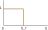
\includegraphics[]{figures/5_1Fermi.pdf}
            \caption{Fermi-Energie ist die Maximalenergie, bis zu der die Zustände bei $T=0$ konstant sind}
            \label{}
        \end{figure}
        \item Für drei Elektronen-Gase sind Flächen konstanter Energie Kugelflächen $\rightarrow$ $E_F^0$ entspricht Kugeloberfläche, die besetzte von unbesetzten Zuständen trennt.\\
         $k_F$ Fermikugelvektor
         \begin{align*}
             &N = \int_0^{E_F^0} D(E)dE = \frac{V}{2\pi^2} (\frac{2m}{\hbar^2})^\frac{3}{2}\frac{2}{3}(E_F^0)^\frac{3}{2}\\
             &\text{mit} \qquad n=\frac{N}{V} \text{ Elektronendichte}\\
            &\Rightarrow \qquad E_{F}^0 = \frac{\hbar^2}{2m} (3 \pi^2 n)^\frac{3}{2}
         \end{align*}
         \item[$\rightarrow$] hängt nur von Dimension und Elektronendichte ab
         \begin{itemize}
             \item[$\rightarrow$] Ein-Parameter-Modell
         \end{itemize} 
         $E_{F}^0 := \frac{\hbar^2 k_F^2}{2 m} \quad \rightarrow \quad k_F = ( 3 \pi^2 n )^{1/3}$ Fermi-Wellenvektor
         \begin{table}[H]
            \centering
             \begin{tabular}{ll}
                 Fermi-Geschwindigkeit & $v_F = \frac{\hbar k_F}{m}$\\
                 Fermi-Wellenlänge & $\lambda_F = \frac{2 \pi}{k_F}$\\
                 Fermi-Temperatur & $T_F = \frac{ E_F^0}{k_B}$\\
                 Zustandsdichte an der \glqq Fermi-Kante\grqq &
                    $D(E_F^0) = \frac{3}{2} \frac{N}{E_F^0}$ \\
                    &$\frac{D(E_F^0)}{V} = \frac{3}{2} \frac{n}{E_F^0}$
             \end{tabular}
         \end{table}

         Beispielwerte:
         \begin{table}[H]
             \centering
             \begin{tabular}{c|ccccc}
                 & $ n (10^{22}cm^{-3}) $ & $k_F ($\AA$^{-1})$ & $v_F (10^6 m/s)$ & $E_F^0 (eV)$ & $T_F (K)$  \\ \hline
            Li  & 4,62 & 1,11 & 1,1  & 4,69  & 54400 \\
            Na  &2,62   &0,91   &1,05   &3,11   &36700\\
            Al  &18,7   &1,75   &2,03   &11,67  &135700\\
            Ag  &5.87   &1.2    &1.39   &5.49   &62700 \\
            Au  &5,9    &1,2    &  1.38  &   5.51    &  63900    \\
                &       &$\approx \frac{1}{a}$  & $\approx 10^6 m/s$    & $\approx 5 eV $   & $T_F \gg T_{Schmelz} $ \\
                &       &                       & $< c$                 & $\gg k_BT$         & $> \Theta_D \approx RT $
            \end{tabular}
         \end{table}
    \end{itemize}
    \item[(ii)] \textbf{Elektronengas bei endlicher Temperatur}
    \begin{align}
        f(E,T) = \frac{1}{e^{\frac{E-\mu}{K_B T}}}
    \end{align} 
    \begin{itemize}
        \item Energieintervall, in dem Umsetzungen möglich sind $\pm 1.75 k_B T$\\
            Da $k_B T_{TR} \approx 25 meV \ll E_F^0 $ ist Tieftemperaturnäherung oft gerechtfertigt für Metalle.
        \item Für $T=0$ ist $\mu(T=0) = E_F^0$ 
        \item Mit N $\overset{!}{=} \int_0^{\infty} D(E) f(E,T) \mathrm{d}E \, \rightarrow \, \mu(T) \approx E_F^0 \left[1-\frac{\pi^2}{12} \left(\frac{T}{T_F}\right)^2 \right]$\\
            Für RT gilt in guter Näherung $\mu(300K) \approx E_F^0 = E_F$
    \end{itemize}


\item[(d)] \textbf{Spezifische Wärme des freien Elektronengases} \\
        Die innere Energie des Fermi-Gases bei $T=0$
        \begin{align}
            U_0 &= \int_0^\infty E D(E)f(E,T=0) \, \mathrm{d}E = \int_0^{E_F^0} E \frac{V}{2\pi^2} \left( \frac{2m}{\hbar^2} \right)^{3/2} \sqrt{E} \mathrm{d}E\\
            &= \frac{V}{2pi^2} \left(\frac{2m}{\hbar}\right)^{3/2} \cdot \frac{2}{5} (E_F^0)^{5/2} = \frac{3}{5} N \cdot E_F^0 = \frac{3}{5} N k_B T_F
        \end{align}
        Energiedichte $ n_0 = \frac{U_0}{V} = \frac{3}{5} n E_F^0 = \frac{3}{5} n k_B T_F$. \\
        Bei endlicher Temperatur
        \begin{align}
            U = \int_0^\infty E D(E) f(E,T) \mathrm{d}E = A\underbrace{\int_0^\infty \frac{E^{\frac{3}{2}}}{e^{\frac{E-\mu}{k_BT}}+1} \mathrm{d}E}_{\text{nicht analytisch lösbar}}
        \end{align}
        Spezifische Wärme $C_V = \left(\frac{\partial U}{\partial T}\right)_V$ \\
        \begin{itemize}
            \item[I] Abschätzung $\delta U(T) = U(T) - U_0$:
            \item[] {\centering
                \fbox{ $\delta U(T) \approx \underset{\text{Energiebetrag}}{k_B T} \cdot \underset{\text{Anzahl}}{N \frac{T}{T_F}} = N k_B \frac{T}{T_F} \, \rightarrow \, C_V = \left(\frac{\partial U}{\partial T}\right)_V = $}
                
            }


            \item[II] Rechnung \\
                Energieaufnahme des Fermi-Gases bei Erwärmung von $T=0$ auf T. \\
                \begin{align}
                    \delta U(T) = \int_0^\infty E D(E) f(E,T) \mathrm{d}E - \int_0^{E_F} E D(E) \mathrm{d}E \label{eq:5_1}
                \end{align} 
                Ferner
                \begin{align}
                    E_F N = E_F \int_0^\infty D(E) f(E,T) \mathrm{d} E \label{eq:5_2}
                \end{align}
                Leite \ref{eq:5_1} und \ref{eq:5_2} nach T ab.
                \begin{align}
                    C_v &= \int_0^\infty E D(E) \frac{\partial f(E,T)}{\partial T} \mathrm{d}E \label{eq:5_3} \\
                    0 &= E_F \int_0^\infty D(E) \frac{\partial f(E,T)}{\partial T} \mathrm{d}E \label{eq:5_4}
                \end{align} 
                Jetzt \ref{eq:5_3} - \ref{eq:5_3}:
                \begin{align}
                    C_v &= \int_0^\infty (E - E_F) D(E) \frac{\partial f(E,T)}{\partial T} \mathrm{d}E \\
                    &\approx D(E_F) \int_0^\infty (E - E_F) \frac{\partial f(E,T)}{\partial T} \mathrm{d}E
                \end{align}
                Wobei in der Abschätzung ausgenutzt wurde, dass $\partial f/\partial T \neq 0 $ nur um $E_F$ gilt. Mit
                \begin{align}
                    \frac{\partial f(E,T)}{\partial T} = \frac{E-E_F}{k_B T^2} \frac{e^{\frac{E-E_F}{k_BT}}}{\left(e^{\frac{E-E_F}{k_BT}} + 1\right)^2}
                \end{align}
                mit $x := \frac{E-E_F}{k_B T}$
                \begin{align}
                C_v = k_B^2 T D(E_F) \int_{-E_F / (k_B T) \rightarrow - \infty}^\infty \frac{x^2e^x}{(e^x+1)^2}\mathrm{d}x
                \end{align}
                {\centering
                \fbox{$ \frac{\pi^2}{3} k_B^2 T D(E_F) = \frac{\pi^2}{2} N k_B \frac{T}{T_F}$}
                }
        \end{itemize}
\begin{align*}
    C_V(T) = \underbrace{\gamma T}_{El.} + \underbrace{\beta T^3}_{Phonon} \qquad &\text{Gesamte spezifische Wärme}\\
    \frac{C_V(T)}{T} = \gamma + \beta T^2 \qquad &\text{geschickte Auftragung zur Best. von $\gamma$ und $\beta$}
\end{align*}
mit $\gamma := \frac{\pi^2}{2}N k_B \frac{1}{T_F}$, $\beta = \frac{12 \pi^4}{5} N k_B \frac{1}{\Theta_D^3}$.\\

\textbf{Diskussion:} \\
Für tiefe Temperaturen $(T \ll \Theta_D)$: Beitrag des Gitters recht klein, da $T^3$-Abhängigkeit. $\rightarrow$ Anteil der Elektronen messbar (siehe Folie) wegen schwächerer T-Abhängigkeit. \\
Für hohe Temperaturen $(T \gg \Theta_D)$: Phononenbeitrag dominiert $C_{Ph} \approx 3 N_A k_B T$. \\
Bemerkung: \\
Modell passt gut ($\approx 25 \%$) für einfache Metalle, schlecht für Übergangsmetalle mit teilweise gefüllten d-Schalen.

\end{itemize}

\subsection{Elektronen im periodischen Potential} \label{kap:5_2}
Potential im Topf hat Translationssymmetrie des Gitters.
%TODO Bild 5_2
\begin{itemize}
    \item[(a)] \textbf{Bloch-Wellen:}\\
    Schrödingergleichung: $-\frac{\hbar^2}{2m} \Delta \Psi(\textbf{r}) + V(\textbf{r}) \Psi(\textbf{r}) = E \cdot \Psi(\textbf{r})$\\
    mit $V(\textbf{r}) = V(\textbf{r} + \textbf{R})$ mit Gittervektor $\textbf{R}$.\\
    Analog: Berechnung Streudichteverteilung $\rightarrow$ Fourier-Darstellung $V(\textbf{r}) = \sum_{\textbf{G}} V_{\textbf{G}} e^{i \textbf{G} \textbf{r}}$ mit reziprokem Gittervektor $ \textbf{G}$. Die Fourierkoeffizienten $V_{\textbf{G}}$ sind charakteristisch für den Kristall. \\
    Ansatz für Wellenfunktion: Entwicklung nach ebenen Wellen
    \begin{align}
        \Psi(\textbf{r}) &= \sum_{\textbf{k}} c_{\textbf{k}} e^{i \textbf{k} \textbf{r}} = \sum_k \Psi_{\textbf{k}}(\textbf{r}) \\
        &=\sum_{\textbf{k}} \frac{\hbar^2 k^2}{2m} C_{\textbf{k}} e^{i \textbf{k} \textbf{r}} + \sum_{\textbf{k'},\textbf{G}} C_{\textbf{k'}} C_{\textbf{k}} e^{i (\textbf{k'} +\textbf{G}) \textbf{r}}\\
        &= E \sum_{\textbf{k}} C_{\textbf{k}} e^{i \textbf{k} \textbf{r}}
    \end{align}
    setzen $k := \textbf{k'} + \textbf{G} $ erlaubt, da über alle $\textbf{k}$, $\textbf{G}$ summiert wird. (entspricht Umsortierung).
    \begin{align}
        \sum_{\textbf{k}} e^{i \textbf{k} \textbf{r}} \left[\left(\frac{\hbar^2k^2}{2m} - E\right)c_{\textbf{k}} + \sum_{\textbf{G}} V_{\textbf{G}} c_{\textbf{k}-\textbf{G}}\right] \overset{!}{=} 0
    \end{align}
    für alle $\textbf{r}$. Somit
    \begin{align}
        \left(\frac{\hbar^2k^2}{2m} - E\right)c_{\textbf{k}} + \sum_{\textbf{G}} V_{\textbf{G}} c_{\textbf{k}-\textbf{G}} = 0
    \end{align}

    \begin{itemize}
        \item Satz algebraischer Gleichungen
        \item Zahl der erlaubten $\textbf{k}$ aus Randbedingungen
        \item Für jedes $\textbf{k}$ existiert ein Gleichungssystem mit Wellenfunktion $\Psi_{\textbf{k}}(\textbf{r})$ und Eigenwert $E_{k}$
        \item Genauso viele Lösungen wie $\textbf{k}$-Werte
        \item Entwicklungskoeffizienten $C_{\textbf{k}}$: ungleich 0, deren Indizes sich um $\textbf{G}$ unterscheiden.
    \end{itemize}

    \begin{align}
        \Psi_{\textbf{k}} (\textbf{r}) &= \sum_{\textbf{G}} c_{\textbf{k}-\textbf{G}} e^{i(\textbf{k}-\textbf{G}) \textbf{r}}\\
        \text{oder} \qquad \Psi_{\textbf{k}} (\textbf{r}) &= \underbrace{\left[\sum_{\textbf{G}} c_{\textbf{k}-\textbf{G}} e^{-i\textbf{G} \textbf{r}}\right]}_{
            \begin{matrix}
                \text{Fourierdarstellung einer} \\ \text{\textbf{R}-periodischen Funktion}\\
                u_{\textbf{k}} ( \textbf{r}) = u_{\textbf{k}} ( \textbf{r} + \textbf{R})
            \end{matrix}
        } e^{i \textbf{k} \textbf{r}}
    \end{align}
    
    $\rightarrow$ Elektronen im periodischen Potential sind Bloch-Wellen mit $u_{\textbf{k}}(\textbf{r}) = u_k(\textbf{r} + \textbf{R})$, $\Psi_{\textbf{k}} (\textbf{r}) = u_k(\textbf{r}) e^{i\textbf{k}\textbf{r}}$. \\
    Eigenschaften von Bloch-Wellen
    \begin{itemize}
        \item[(i)] Bloch-Wellen, die sich um $ \textbf{G} $ unterscheiden, sind identisch.
        \item[(ii)] Eigenwerte $E_{\textbf{k}}$ deren $ \textbf{k} $ sich um $ \textbf{G} $ unterscheiden, sind identisch. $\rightarrow$  $E_{\textbf{k}} = E_{\textbf{k}+\textbf{G}}$
        \item[(iii)]
        \begin{itemize}
            \item Die elektrischen Eigenschaften $\Psi_{\textbf{k}} (\textbf{r})$ und Eigenwerte $E_k$ wiederholen sich im $\textbf{k}$-Raum periodisch.
            \item Betrachtung in einer Einheitszelle des $\textbf{k}$-Raums ausreichend $\rightarrow$ 1. BZ.
        \end{itemize}
    \end{itemize}
    \item[(b)] \textbf{Modell des leeren Gitters}\\
    Annahme: Amplitude des periodischen Potentials so klein, dass dieses vernachlässigt werden kann. $V_{\textbf{G}}\approx 0$, aber trotzdem Gitterperiodizität vorliegt.\\
    Aus (*) folgt: $ E_{\textbf{k}} = \frac{\hbar^2k^2}{2m} = \frac{\hbar^2}{2m} \left|\textbf{k}+\textbf{G}\right|^2 = E_{\textbf{k} + \textbf{G}}$ \\
    $\rightarrow$ Energieeigenwerte sind Parabeln im $\textbf{k}$-Raum, die sich um reziproken Gittervektor $\textbf{G}$ unterscheiden. \\
    \textbf{Beispiel}: 1D Gitter mit Gitterkonstante a, ausgedehntes Zonenschema \\ %TODO Bild 5.2b
    Reduziertes Zonenschema: Durch Verschieben der Parabeln von außerhalb in die 1. BZ (Addieren von $\textbf{G}$) \\ %TODO noch ein Bild 5.2c
    $\rightarrow$ zu jedem \textbf{k}-Vektor gibt es mehrere $E_k$. \\
    \textbf{Beispiel}: 3D kubisch primitives Gitter
    \begin{align}
        E_{\textbf{k}} = \frac{\hbar^2k^2}{2m} = \frac{\hbar^2}{m^2}\left[(k_x+G_x)^2 + (k_y+G_y)^2 + (k_z+G_z)^2\right] = E_{\textbf{k}+\textbf{G}}
    \end{align}
    \begin{itemize}
    \item[$\rightarrow$] 3D-Anordnung von Parabeln
    \item[$\rightarrow$] Auftreten von Entartung: vor allem bei hohen Energien fallen Parabeläste zusammen. $\rightarrow$ mehrere k-Zustände mit gleicher Energie im leeren Gitter
    \item[$\rightarrow$]] aufgehoben durch Hinzunahme eines endlichen Potentials $\rightarrow$ 
    \end{itemize}

    \item[(c)] \textbf{Modell fast freier Elektronen} \\
    Annahme: periodisches Potential so schwach, dass Elektronen sich nahezu frei durch den Kristall bewegen $\rightarrow$ gutes Modell für Leitungselektronen in Metallen, beschreibt das Auftreten von \textbf{Bandlücken}.
    \begin{itemize}
        \item[(i)] \textbf{Motivation:} Betrachte Bewegung eines Elektrons entlang 1D Atomkette. Elektron wir an Atomen gestreut: Bedingung für Bragg-Reflex: $\Delta \textbf{k} = \textbf{G}$. \\
        1D: Rückreflexion der einlaufenden Welle $\Delta \textbf{k} =  \textbf{k}' -  \textbf{k} = 2 \textbf{k} $. Auftreten der Bragg-Reflexion für $k = \pm G/2 = \frac{2\pi}{2a}\cdot n = \frac{\pi}{a} n \quad (n \in \mathrm{N}) \quad k_{min} = \frac{\pi}{a}$. \\
        In diesem Fall überlagern sich einlaufende und gestreute Welle zu stehender Welle
        \begin{align}
            \Psi_{s,a} \propto e^{i\pi \frac{x}{a}} \pm e^{-i\pi \frac{x}{a}} = \begin{cases}
                cos(\frac{\pi x}{a}) & \text{für } s \\
                sin(\frac{\pi x}{a}) & \text{für } a 
            \end{cases}
        \end{align}
        $\rightarrow$ Räumlich modulierte Ladungsdichte:
        \begin{align}
            \rho_{s,a} = e \left|\Psi_{s,a}\right|^2 \propto \begin{cases}
                cos(\frac{\pi x}{a}) & \text{für } s \\
                sin(\frac{\pi x}{a}) & \text{für } a 
            \end{cases}
        \end{align}
        (Vergleiche: laufende ebene Welle ist räumlich konstant.)\\
        Braggreflexion am Rand der 1. BZ für $k_{???} = \pm \frac{\pi}{a}$\\
            $\rightarrow$ stehende Welle mit $\rho_s$ und $\rho_a$.\\
            $\rho_{s,a}$ hat hohe/niedrige Ladungsdichte an Ort der Inonen. Gesamtenergie für $\Psi_{s,a}$ niedriger/höher\\
            $\rightarrow$ Aufspaltung in ??? \textbf{Energiebänder} durch Aufhebung der Entartung $E_{s,a}$ abgesenkt/erhöht.  
            \item[(ii)] \textbf{Berechnung der Energielücke am Rand der BZ:}\\
            \begin{itemize}
                \item Rand der BZ ($k = \frac{\pi}{a}$) Schnittpunkt zweier Energieparabeln: $E_{\textbf{k}}$ und $E_{\textbf{k}-\textbf{G}_0}$
                \item Schwaches Potential: Zwei-Komponenten-Näherung: 1. und 2. BZ reicht aus.
                \begin{align*}
                    \Psi(\textbf{r}) = c_{\textbf{k}} e^{i \textbf{k} \textbf{r}} + c_{\textbf{k}-\textbf{G}_0} e^{i(\textbf{k}-\textbf{G}_0) \textbf{r}}
                \end{align*}
                Aus (???) zur ??? Gleichungen
                \begin{align*}
                    \left(\frac{\hbar^2 k^2}{2m}-E\right) c_{\textbf{k}} + V_{\textbf{G}_0} c_{\textbf{k}-\textbf{G}_0} &= 0\\
                    \left(\frac{\hbar^2 \left|\textbf{k}-\textbf{G}_0\right|^2}{2m}-E\right) c_{\textbf{k}-\textbf{G}_0} + V_{-\textbf{G}_0} c_{\textbf{k}} &= 0
                \end{align*}
                mit dem Inversionssymmetrischen Filter $V_{-\textbf{G}_0} = V_{\textbf{G}_0}$.\\
                Lösung liefert
                \begin{align*}
                    E_{s,a} = E_{\textbf{k}}^0 \mp \left|V_{\textbf{G}_0} \right| \, , \quad E_a-E_s=2 \left|V_{\textbf{G}_0}\right|
                \end{align*}
                Verlauf der Dispersion am Rand der BZ: $E_{s,a} \sim \pm \left| k - \frac{G_0}{2} \right|^2$\\
                \begin{itemize}
                    \item[$\rightarrow$] negative Krümmung von $\Psi_s$ entspricht negativer Masse.
                    \item Tief in BZ keine Änderung, Änderungen am Rand der BZ.
                    \item Auftreten von Energiebändern (erlaubte Energiebereiche) und dazwischen Bandlücke (verbotener Energiebereich)
                    \item ???
                \end{itemize}
            \end{itemize}
        \end{itemize}
    \item[(d)] \textbf{Modell stark gebundener Elektronen (Tight binding Modelle)} \\
    \textbf{Annahme:} Es sei in der Nähe der Atomrümpfe lokalisiert. Beschreibung der Zustände durch Atomorbitale (Linear Combination of Atomic Orbitals / LCAO) (vgl. Bindungstypen).\\
    \begin{itemize}
        \item Ein-Elektron-Näherung Gitterpotential als Summe der Atompotentiale $V_A(r)$ Potential des Bezugatoms und ein Störpotential durch alle anderen Kristallatome
        \item Energieeigenwerte aus Rityschem Verfahren \begin{align*}
            E_{\textbf{k},i} = \frac{\int \Psi_{\textbf{k},i}^* H \Psi_{\textbf{k},i} \mathrm{d}r}{\int \Psi_{\textbf{k},i}^* \Psi_{\textbf{k},i} \mathrm{d}r}
        \end{align*}
        ist angenäherte Wellenfunktion.
        \begin{align*}
            \Psi_{\textbf{k},i}\approx \Phi_k = \underset{\begin{matrix}
                \uparrow\\
                \text{Anzahl}\\
                \text{Atome}
            \end{matrix}}{\frac{1}{\sqrt{N_A}}}\sum_m \underset{\begin{matrix}
                \uparrow\\
                \text{atomare}\\
                \text{Wellenfkt.}
            \end{matrix}}{\Psi^0_i(\textbf{r}-\textbf{R}_m)}\cdot \underset{\begin{matrix}
                \uparrow\\
                \text{Blochwellen}
            \end{matrix}}{e^{i \textbf{k} \textbf{R}_m}}
        \end{align*}
        \item Annahme: einfach kubisch, 1-atomige Basis,nächste Nacharn 
        \begin{align*}
            E_{k,i} \approx  \underset{\begin{matrix}
                \text{Eigenwert des}\\
                \text{isolierten Atom}           \end{matrix}}{E_i} - A_i - 2B_i[\cos(k_x a)+ \cos(k_y a) + \cos(k_z a)]
        \end{align*}
        \begin{table}[H]
            \begin{tabular}{cc}
                $E_i$ & Eigentwert des isolierten Atom\\
                $A_i$ & ??? \\
                $B_i$ & durch Überlapp der Wellenfunktion $\int \Psi^* \Psi \mathrm{d}r$
            \end{tabular}
        \end{table}
        \begin{itemize}
            \item[(1)] Wechselwirkung der  $N_A$ Atome $\rightarrow$ Aufspaltung der Energieniveaus in $N_A$ quasikontinuierliche Zustände, aus diskreten Energien werden \textbf{Energiebänder}.
            \item[(2)] Mittlere Verschiebung des Energieniveaus i (Lage der Bandmitte ist $A_i$: $A_i > 0$ $\rightarrow$ Absenkung
            \item[(3)] $A_i$ durch Potential der Nachbaratome, nimmt zu für abnehmenden Gitterabstand a, Absenkung am stärksten für kleine a.
            \item[(4)] Breite des Bandes ist $\alpha$ $B_i$. Für sc: Bandbreite $\pm 6 B_i$
            \item[(5)] $B_i$ bestimmt durch Überlappintegral, Tiefliegende Zustände haben schmale Bänder, da Überlapp gering
            \item[(6)] In der Mitte der BZ ($\textbf{k} = 0$). $E_{k,i} (k) = E_i A_i - 6 B_i + B_i a^2k^2$
            $\rightarrow$ näherungsweise quadratische Dispersion\\
            mit effektiver Masse $m_i^* = \frac{\hbar^2}{\sum B_i a^2}$ durch Überlapp der Wellenfkt.
            \item[(7)] Bandindex an Atomorbitalen
            \item[(8)] Jedes Band kann gemäß Pauliprinzip $2N_A$ Elektronen aufnehmen 
        \end{itemize}
    \end{itemize}
\end{itemize}
